% Author: Adolfo Centeno 
% Kubeet Corp
% www.kubeet.com

 
\documentclass{beamer}
\setbeamertemplate{navigation symbols}{}
\usepackage[utf8]{inputenc}
\usepackage{beamerthemeshadow}
\usepackage{listings}

\begin{document}

\title{Angular - Integration testing - Team lider}  
\author{Adolfo Centeno}
\date{\today} 

\begin{frame}
\titlepage

\end{frame}

\begin{frame}\frametitle{Table of contents}\tableofcontents
\end{frame} 


\section{install Angular - Testing Intro} 


\defverbatim[colored]\lstjenkins{
 \begin{lstlisting}[language=bash,showstringspaces=false, basicstyle={\tiny}, keywordstyle=\color{red}]
node {
    stage('Checkout') {
        checkout scm
    }
    stage('Build') {
        docker.image('trion/ng-cli').inside {
            sh 'npm install'
            sh 'ng build --progress false --prod --aot'
            sh 'tar -cvzf dist.tar.gz --strip-components=1 dist'
        }
        archive 'dist.tar.gz'
    }
    stage('Test') {
        docker.image('trion/ng-cli-karma').inside {
            sh 'ng test --progress false --watch false'
        }
    }
}
 \end{lstlisting}
}



\begin{frame}\frametitle{} 


\begin{block}{open new terminal, install Angular}
sudo npm install -g @angular/cli
\end{block}

\begin{block}{create repo}

\url{https://github.com} \\
name: angular-integration-testing

\end{block}


\begin{block}{create angular project}
ng new angular-integration-testing \\
cd angular-integration-testing \\
ng serve --open \\
ng test
\end{block}

\end{frame}


\begin{frame}\frametitle{} 

\begin{block}{git init, master branch}
git init \\
git remote add origin https://github.com/your-user-lider/angular-integration-testing.git \\
git add . \\

git commit -m "add initial master" \\
git push -u origin master
\end{block}

\begin{block}{develop branch}
git branch develop \\
git checkout develop \\
git branch \\
git merge master develop 
\end{block}

\end{frame}



\begin{frame}\frametitle{} 

\begin{block}{nano Jenkinsfile}
\lstjenkins
\end{block}

\begin{block}{push develop branch}
git add . \\
git commit -m "add initial develop" \\
git push -u origin develop
\end{block}

\end{frame}



\begin{frame}\frametitle{} 

go to trello \url {https://trello.com/}

\begin{itemize}
\item create a board
\item invite to your team members
\item create the cards voter, todos, users
\item each developer should edit his card 
\item link your board to github repo
\item link each card to branch develop
\end{itemize}

\end{frame}


\begin{frame}\frametitle{} 

\begin{block}{Go to jenkins url}
\url{http://35.227.59.176} \\
user:  adsoftsito \\
passwd:  5i5i5i5i

\end{block}

\end{frame}


\begin{frame}\frametitle{} 

\begin{block}{create new item}
\begin{itemize}
\item type name :  team-integration-testing 
\item choose Pipeline Project
\end{itemize}
\end{block}

\begin{center}
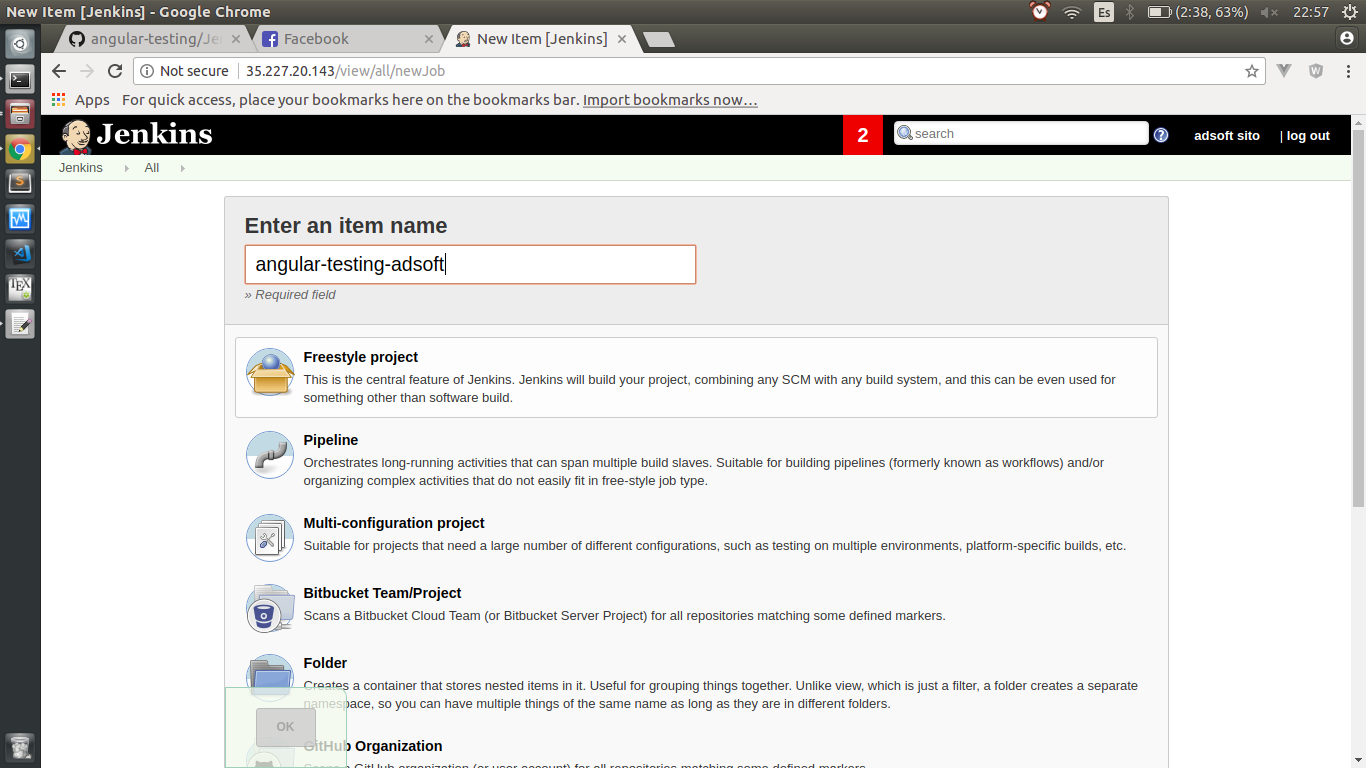
\includegraphics[width=0.9\textwidth]{jenkins-newitem.png}
\end{center}

\end{frame}



\begin{frame}\frametitle{} 

\begin{block}{create new item}
\begin{itemize}
\item put github url
\end{itemize}
\end{block}


\begin{center}
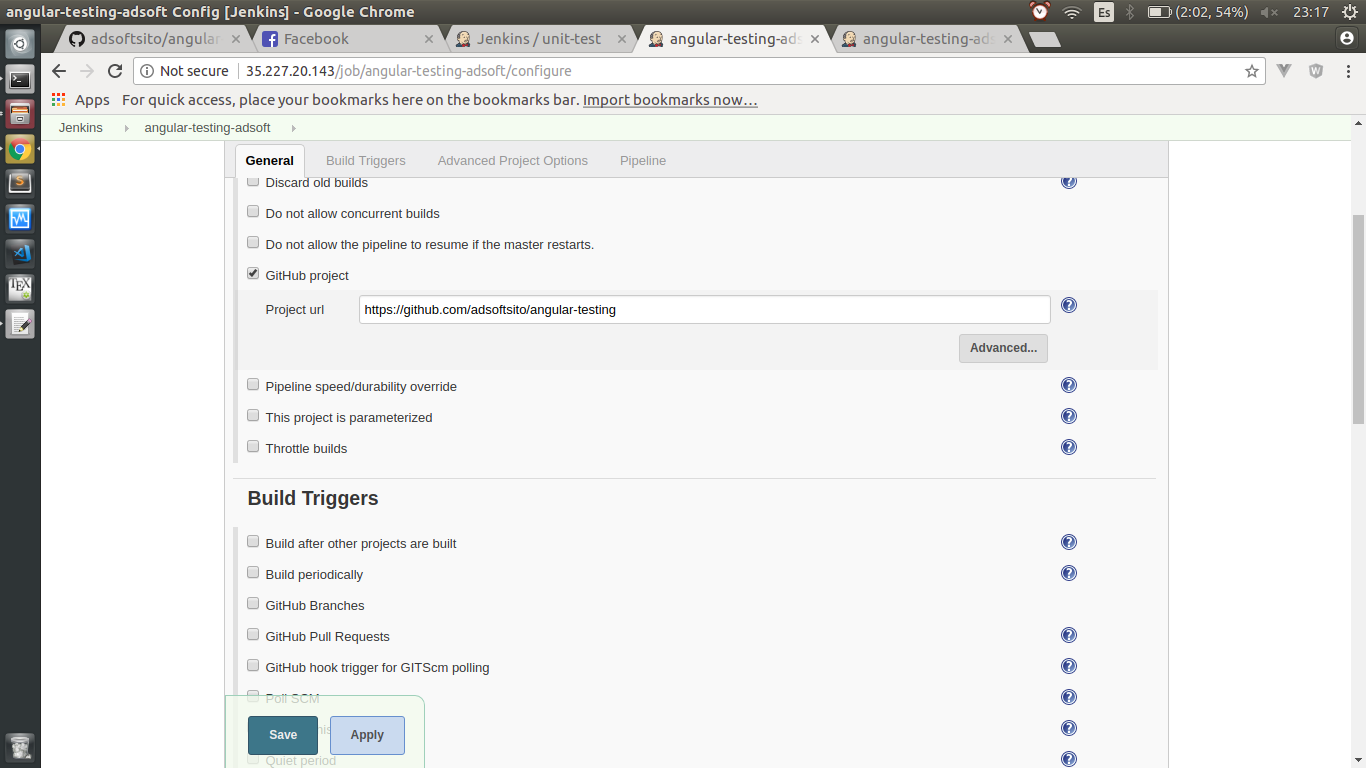
\includegraphics[width=0.9\textwidth]{jenkins-github.png}
\end{center}

\end{frame}



\begin{frame}\frametitle{} 

\begin{block}{create new item}
\begin{itemize}
\item select pipeline from SCM
\item select branch develop
\end{itemize}
\end{block}


\begin{center}
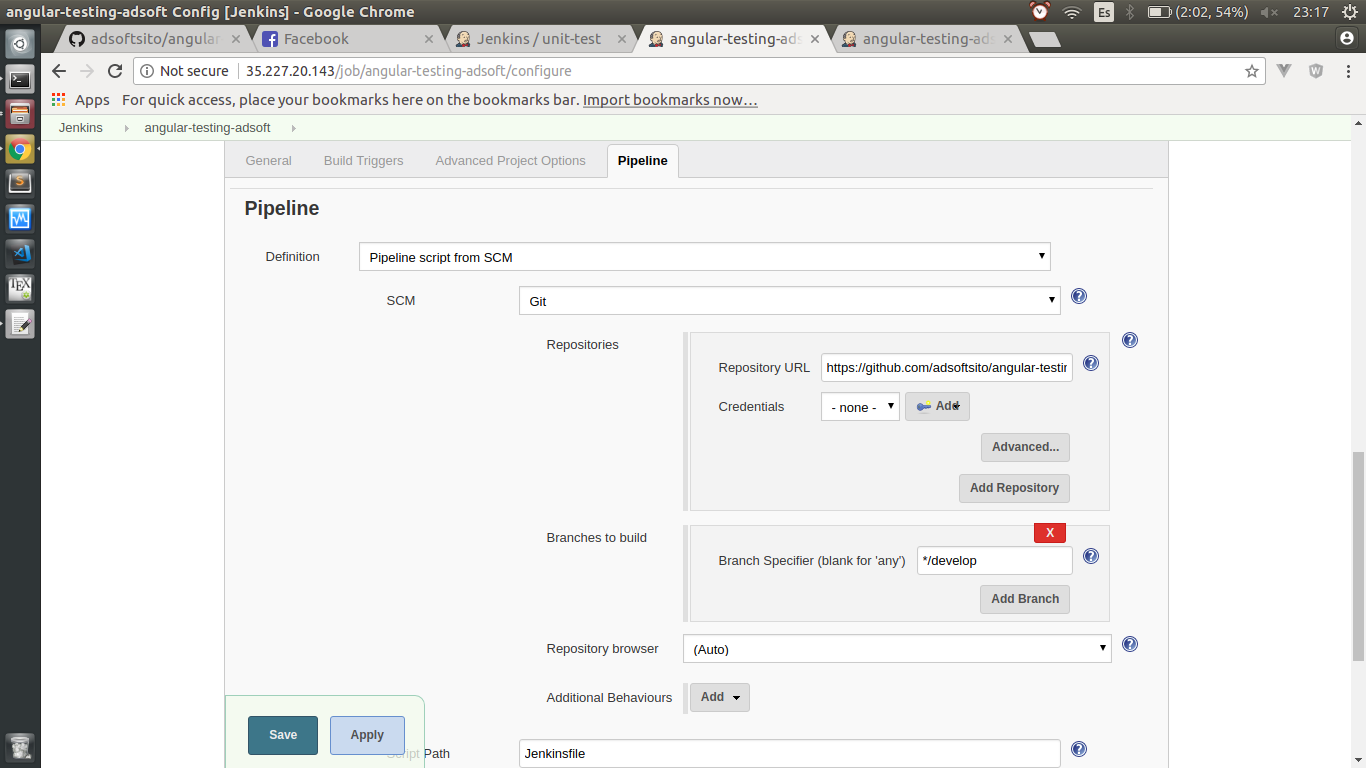
\includegraphics[width=0.9\textwidth]{jenkins-pipeline.png}
\end{center}

\end{frame}


\begin{frame}\frametitle{} 

\begin{block}{open blue ocean}
\begin{itemize}
\item open blue ocean
\end{itemize}
\end{block}


\begin{center}
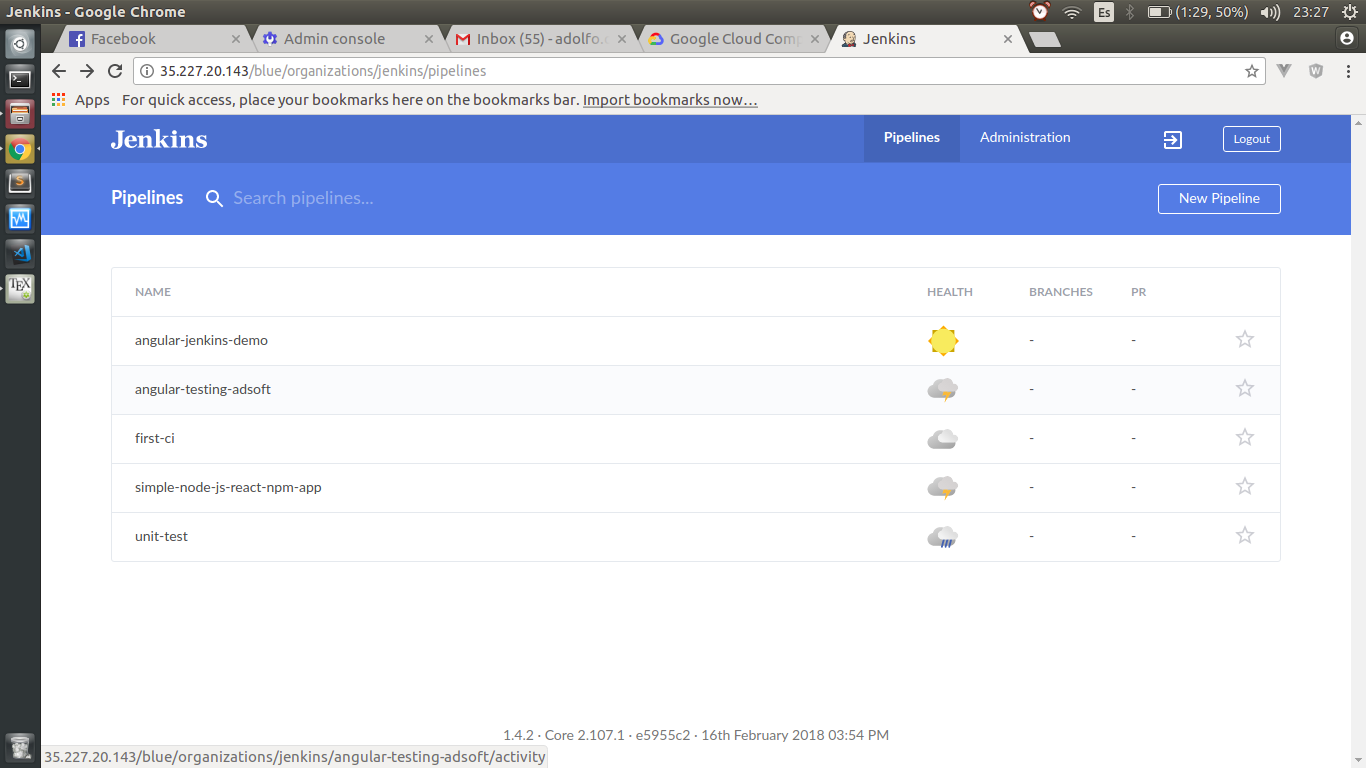
\includegraphics[width=0.9\textwidth]{jenkins-blue-ocean.png}
\end{center}

\end{frame}



\begin{frame}\frametitle{} 

\begin{block}{run job}
\end{block}


\begin{center}
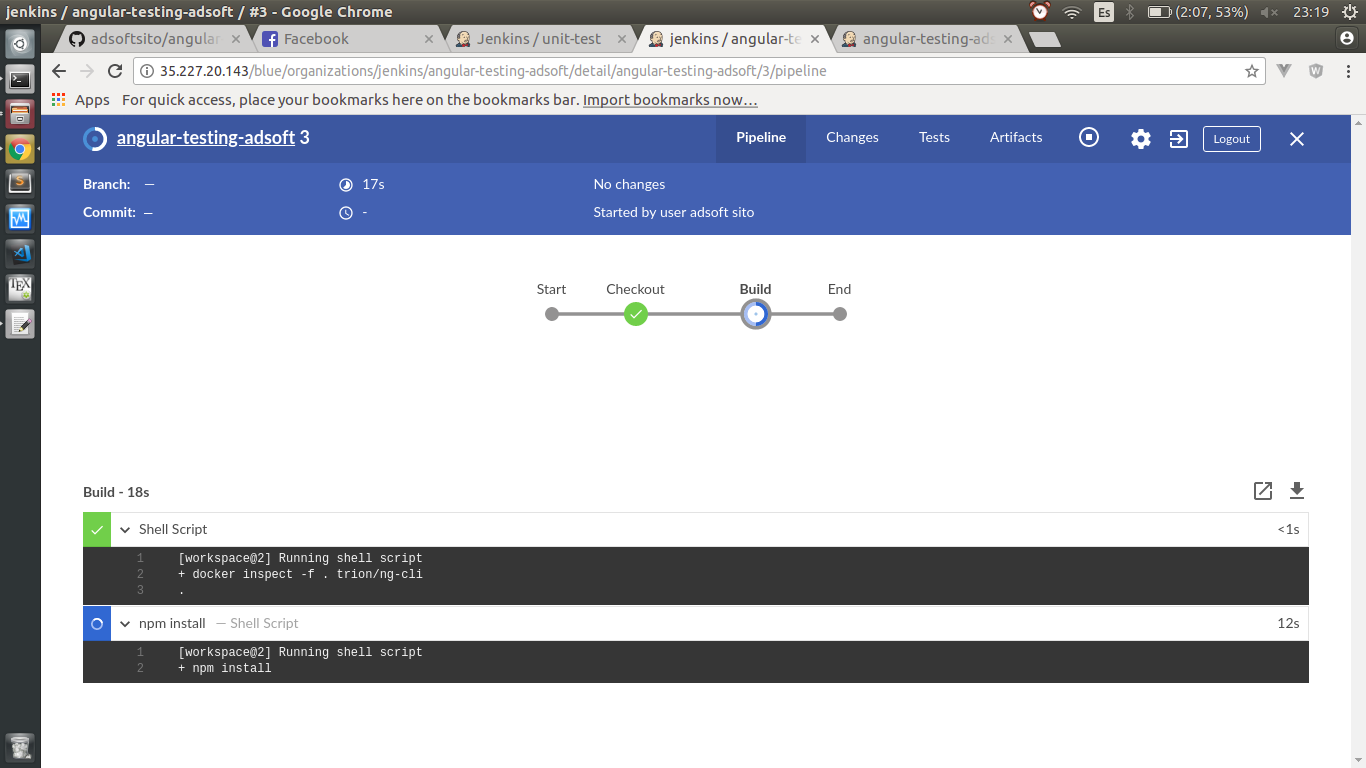
\includegraphics[width=0.9\textwidth]{jenkins-build.png}
\end{center}

\end{frame}



\begin{frame}\frametitle{} 

\begin{block}{run job}
\end{block}


\begin{center}
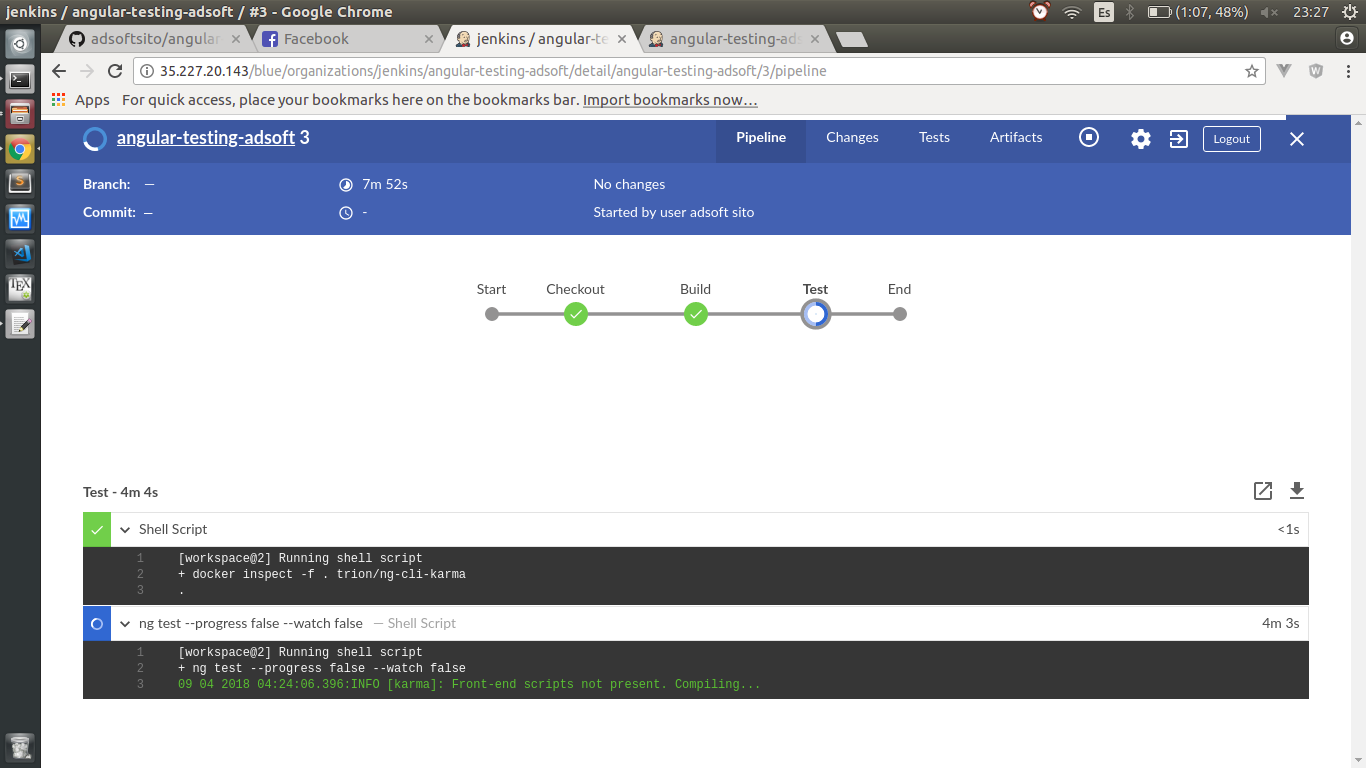
\includegraphics[width=0.9\textwidth]{jenkins-testing.png}
\end{center}

\end{frame}
\end{document}
